\chapter{Introducción}
\label{sec:introduction}

Se sabe que el rendimiento de cualquier empresa está intrínsecamente ligado al factor humano que la conforma (\cite{krekel2019employee}). Por lo tanto, mantener la satisfacción y motivación de los empleados dentro de la organización es un desafío constante que requiere una atención continua. La satisfacción de los trabajadores abarca varios aspectos cruciales para su bienestar y desempeño en el entorno laboral, siendo la seguridad y salud laboral los más prioritarios. Garantizar un ambiente laboral seguro y saludable no solo promueve el bienestar físico y emocional de los empleados, sino que también contribuye significativamente a la productividad y eficiencia general de la empresa. \par
Es responsabilidad de toda organización garantizar la seguridad y salud en el trabajo tanto para sus empleados como para cualquier otra persona que pueda verse afectada por sus operaciones (\cite{Bolivia1979}). La implementación de un Sistema de Gestión de la Salud y Seguridad en el Trabajo(SST) tiene como meta principal proporcionar un entorno laboral seguro y saludable, prevenir lesiones y problemas de salud relacionados con el trabajo, y mejorar continuamente el desempeño en SST.\par
La Norma Técnica de Seguridad (NTS) Nº 009/23, aprobada en Bolivia en 2023, establece las directrices de obligatorio cumplimiento para la presentación y aprobación de los Programas de Gestión de Seguridad y Salud en el Trabajo(PGSST). El PGSST tiene la finalidad de prevenir los riesgos laborales, accidentes de trabajo y enfermedades ocupacionales, a través de la gestión e implementación de mecanismos y medidas en el marco de la normativa legal vigente.\par
La implementación efectiva del PGSST sigue siendo un desafío debido a varios factores, incluyendo la falta de conciencia sobre la importancia de la SST, la resistencia de algunos sectores empresariales y la falta de recursos para la implementación de las medidas requeridas. Aunque la normativa establece claramente la obligatoriedad de su cumplimiento, muchas empresas aún no se han adaptado al nuevo mecanismo, lo que las expone a multas y sanciones.\par
Además de las estrategias tradicionales para mejorar la seguridad y salud en el trabajo, como la identificación y evaluación de riesgos, capacitaciones, equipos de protección personal (EPP), controles de ingeniería y la promoción de una cultura de seguridad; La implementación de sistemas de gestión de la SST no solo promueve un entorno laboral más seguro y saludable, sino que también impulsa la eficiencia y la efectividad organizacional. Sin embargo, en un mundo cada vez más impulsado por la tecnología, es crucial considerar cómo la Inteligencia Artificial está revolucionando diversas áreas como el desarrollo de software, la atención médica (\cite{Ellahham2020}) o el campo de la Salud y Seguridad Ocupacional (SySO) (\cite{Jarota2023}). La capacidad de la Inteligencia Artificial (IA) para analizar grandes cantidades de datos, identificar patrones y realizar predicciones precisas la convierte en una herramienta invaluable en estos y otros campos, transformando la forma en que se llevan a cabo tareas y se toman decisiones. 
%-----------------------------------------------------------------------------------------------------------------------------
\section{Planteamiento del Problema}
La falta de identificación proactiva de riesgos laborales, la complejidad en la generación
de PGSST, las deficiencias en capacitación y los desafíos de cumplimiento normativo constituyen el núcleo de un problema multifacético que afecta tanto a la seguridad como al rendimiento general de una empresa. Estos problemas están interconectados y se alimentan mutuamente, creando un ciclo de dificultades que comprometen la salud y seguridad de los empleados, así como la eficiencia operativa de la organización.
%Añadir contexto de los OSH en el mundo

La complejidad en la generación de PGSST se debe en primer lugar a que estos programas deben abarcar una amplia gama de aspectos, que incluyen la comprensión del entorno laboral, el liderazgo en seguridad y salud ocupacional, y la implementación de comités o coordinadores especializados. Además, deben cumplir con una serie de normativas legales, cuya complejidad y cambio constante pueden dificultar su seguimiento. Por último, la generación de un PGSST también conlleva costos que pueden ser prohibitivos para empresas con recursos limitados. En resumen, la complejidad en la generación de los PGSST se debe a la amplitud de aspectos que deben contemplar, la complejidad y cambio constante de las normativas legales que deben cumplir, y los costos asociados a su generación y mantenimiento.

La ausencia de identificación proactiva de riesgos laborales surge de una falta de conciencia tanto por parte de los empleados como de la gestión sobre los peligros inherentes a sus actividades laborales. Esta falta de conciencia puede derivar en una falta de enfoque en la seguridad, lo que aumenta la probabilidad de accidentes y lesiones laborales. A su vez, la complejidad en la generación de PGSST dificulta aún más la mitigación de estos riesgos, ya que las empresas pueden enfrentar obstáculos para desarrollar e implementar medidas preventivas efectivas.

Las deficiencias en capacitación agravan esta situación al limitar la capacidad de los empleados para identificar y responder adecuadamente a los riesgos laborales. La falta de recursos, tanto en términos de personal como de financiamiento, también contribuye a este problema al dificultar la implementación de programas de seguridad robustos y la asignación de los recursos necesarios para abordar adecuadamente la gestión de riesgos laborales.

Además, la complejidad de la legislación relacionada con la salud y seguridad laboral representa un desafío adicional. Las regulaciones cambiantes y la dificultad para comprender y cumplir con estas normativas pueden aumentar los costos adicionales en la gestión de accidentes y la salud de los empleados, así como contribuir al incumplimiento normativo.

En resumen, la falta de identificación proactiva de riesgos laborales, la complejidad en la generación de PSST, las deficiencias en capacitación, la falta de conciencia sobre riesgos laborales, la complejidad de la legislación y la falta de recursos crean un entorno laboral propenso a accidentes, lesiones y problemas de salud, lo que resulta en una baja productividad, costos adicionales y riesgos legales para la empresa. Estos problemas deben abordarse de manera integral para promover un entorno laboral seguro y saludable, así como para mejorar la eficiencia y la efectividad organizacional.

% TODO: Se requiere datos de encuestas a consultoras SySO sobre PGSST para justificar el proyecto

%-----------------------------------------------------------------------------------------------------------------------------
\section{Motivación}

Tomando en cuenta el precedente de dificultades históricas y culturales que han afectado la implementación efectiva de medidas de seguridad y salud en el trabajo en Bolivia, es crucial abordar estos desafíos con una perspectiva renovada y proactiva. La motivación para mejorar las condiciones laborales y promover un entorno seguro y saludable no solo es una responsabilidad ética, sino que también es fundamental para el bienestar y el rendimiento general de la sociedad boliviana.

La Figura \ref{pics:share_of_industry_exposed_to_automation_ai_gs} muestra claramente cómo la automatización y la inteligencia artificial están transformando rápidamente varios sectores de la industria a nivel mundial. Destacándose el potencial de ser automatizadas las tareas administrativas y legales. De acuerdo a \textcite{hatzius2023potentially}, en estas areas hasta un 46\% de las tareas pueden ser automatizadas. Este cambio tecnológico no solo redefine los roles laborales, sino que también plantea nuevas exigencias. En términos de seguridad y salud ocupacional, la aplicación de estas tecnologías a la realidad nacional tiene el potencial para superar obstáculos externos, asi como carencia de recursos y el correspondiente seguimiento que se dificulta en esta región.  

\begin{figure}[htb]
	\centering
	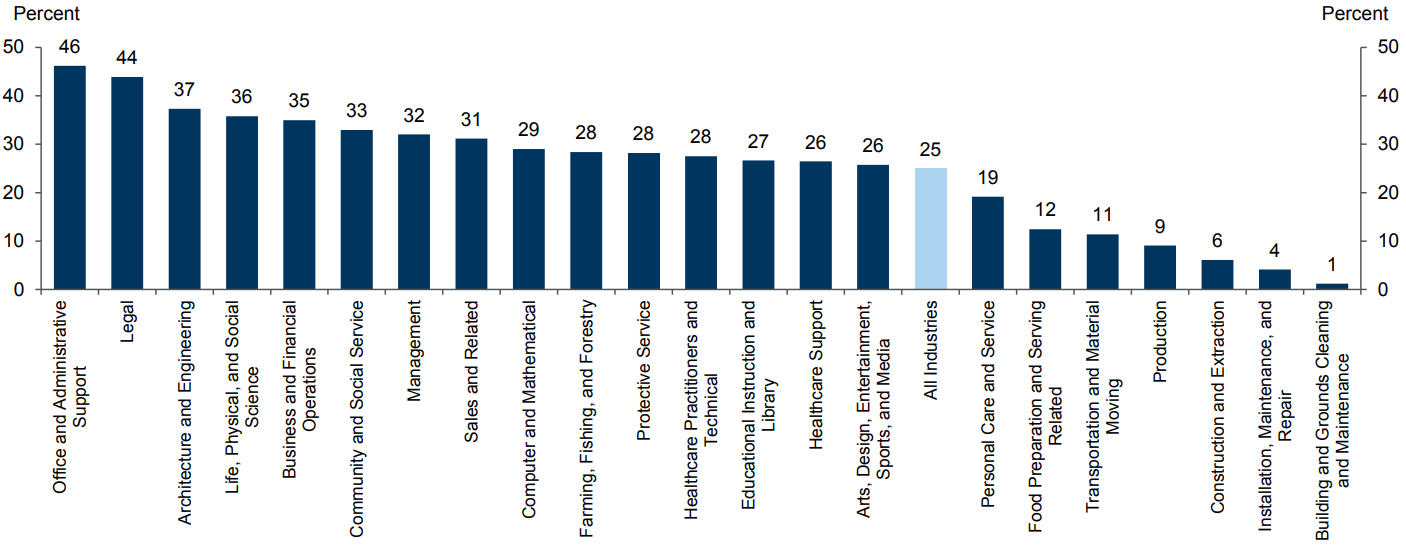
\includegraphics[width=\textwidth]{images/marcoref/share_of_industry_exposed_to_automation_ai.png}
	\caption{Porcentaje de la industria expuesta a la automatización por parte de la IA en Estados Unidos} \vspace{-0.2cm}
	\footnotesize{\textbf{Fuente:} Goldman Sachs Global Investment Research.}
	\label{pics:share_of_industry_exposed_to_automation_ai_gs} 
\end{figure}

En este sentido, utilizar las herramienta de IA para mejorar las condiciones de trabajo y promover la seguridad y salud ocupacional no solo es una necesidad imperativa en el contexto actual de cambio tecnológico y evolución industrial, sino que también es un factor determinante en la construcción de una cultura organizacional sólida y orientada al bienestar integral de sus miembros.

%-----------------------------------------------------------------------------------------------------------------------------

\section{Definición del Problema}
%Se trata de abordar la falta de identificación proactiva de riesgos laborales, la complejidad en la generación de PGSST, las deficiencias en capacitación y preparación contra riesgos de pequeñas y medianas empresas y los desafíos de cumplimiento normativo, así como también facilitar el trabajo de los profesionales de Salud y Seguridad. 
¿Cómo desarrollar un software que identifique de manera efectiva los riesgos laborales y facilite el desarrollo y la gestión eficiente de un PGSST?

%-----------------------------------------------------------------------------------------------------------------------------
\section{Objetivos}
\subsection{Objetivo general}
Implementar un sistema automatizado tomando de base la NTS-009/23 que permita la identificación de riesgos laborales facilitando el desarrollo y la gestión eficiente de PGSST.

\subsection{Objetivos específicos}
\begin{itemize}
    \item Analizar los procesos que se deben seguir para desarrollar los 13 documentos solicitados por la NTS-009/23.
    \item Implementar sistema automatizado de detección de riesgo basado en imágenes y descripciones de texto.
    \item Ofrecer la capacidad de generar automáticamente el PGSST requeridos para cumplir con las regulaciones de seguridad laboral.
    \item Diseñar una interfaz amigable para dispositivos móviles que permita a los usuarios acceder y gestionar la información de seguridad laboral.
\end{itemize}

%-----------------------------------------------------------------------------------------------------------------------------
\section{Justificación}
\subsection{Justificación legal}
La justificación legal de este proyecto se fundamenta en el marco normativo vigente en Bolivia, específicamente en la NTS-009/23, la Ley General de Higiene, Seguridad Ocupacional y Bienestar y otras regulaciones relacionadas.

En primer lugar, la NTS-009/23 establece claramente los requisitos que deben cumplir todas las empresas y lugares de trabajo, tanto nacionales como extranjeros, en relación con la seguridad y salud ocupacional. Esta normativa especifica la obligación de desarrollar y mantener Programas de Gestión de Salud y Seguridad en el Trabajo (PGSST) que garanticen un entorno laboral seguro y saludable para todos los trabajadores. Por lo tanto, la implementación de un sistema automatizado para la gestión de la seguridad y salud ocupacional se justifica en el contexto de cumplimiento de esta normativa, ya que facilitará el cumplimiento de los requisitos establecidos y mejorará la eficiencia en la gestión de los PGSST.

Además, la Ley General de Higiene, Seguridad Ocupacional y Bienestar establece disposiciones generales sobre la protección de la salud y seguridad de los trabajadores en Bolivia. Esta ley tiene como objetivo principal prevenir accidentes y enfermedades ocupacionales, promover condiciones de trabajo seguras y saludables, y garantizar el bienestar general de los trabajadores. En este sentido, la implementación de un sistema automatizado para la gestión de la seguridad y salud ocupacional se alinea con los principios y objetivos establecidos en esta ley, contribuyendo a fortalecer el cumplimiento de las disposiciones legales y a proteger los derechos y la integridad de los trabajadores en el país.

En conclusión, la justificación legal de este proyecto se sustenta en la necesidad de cumplir con la normativa vigente en materia de seguridad y salud ocupacional en Bolivia, específicamente en la NTS-009/23 y la Ley General de Higiene, Seguridad Ocupacional y Bienestar. La implementación de un sistema automatizado para la gestión de la seguridad y salud ocupacional ayudará a garantizar el cumplimiento de los requisitos legales establecidos, promoverá un entorno laboral seguro y saludable, y protegerá los derechos y el bienestar de los trabajadores en el país.

\subsection{Justificación tecnológica}

La justificación tecnológica de este proyecto radica en la necesidad de aprovechar las ventajas de la Inteligencia Artificial (IA) y las tecnologías de información para mejorar la eficiencia y la efectividad en la gestión de la seguridad y salud ocupacional en las empresas bolivianas.

La implementación de un sistema automatizado basado en IA permitirá identificar proactivamente riesgos laborales, agilizar el desarrollo de Programas de Gestión de Salud y Seguridad en el Trabajo (PGSST) y facilitar la gestión eficiente de los mismos. Esta tecnología proporcionará capacidades avanzadas para analizar grandes cantidades de datos, identificar patrones y tendencias, y realizar predicciones precisas, lo que permitirá una toma de decisiones más informada y rápida en materia de seguridad y salud ocupacional.

Además, el uso de tecnologías móviles y aplicaciones web facilitará el acceso a la información de seguridad laboral desde cualquier lugar y en cualquier momento, lo que mejorará la comunicación y la colaboración entre los diferentes actores involucrados en la gestión de la seguridad y salud ocupacional.

En resumen, la adopción de tecnologías de IA y automatización en la gestión de la seguridad y salud ocupacional ofrece una oportunidad única para mejorar la seguridad de los trabajadores, reducir los riesgos laborales y promover un entorno laboral más seguro y saludable en las empresas bolivianas. Esta justificación tecnológica respalda la necesidad de desarrollar e implementar un sistema automatizado para la gestión de la seguridad y salud ocupacional en el contexto específico de Bolivia.

\subsection{Justificación social}

La justificación social de este proyecto se basa en el impacto positivo que tendrá en la sociedad boliviana al mejorar las condiciones de trabajo y promover un entorno laboral seguro y saludable para todos los trabajadores.

La implementación de un sistema automatizado para la gestión de la seguridad y salud ocupacional beneficiará directamente a los trabajadores al reducir los riesgos laborales y prevenir accidentes y enfermedades relacionadas con el trabajo. Esto contribuirá a mejorar su calidad de vida, proteger su integridad física y emocional, y promover su bienestar general.

Además, un entorno laboral seguro y saludable también tendrá un impacto positivo en la productividad y la eficiencia de las empresas, lo que a su vez beneficiará a la economía en general. Menos accidentes y enfermedades laborales significan menos días de trabajo perdidos, menores costos de atención médica y una fuerza laboral más comprometida y motivada.

En última instancia, la implementación de este sistema contribuirá a construir una cultura de seguridad y salud ocupacional en Bolivia, donde la protección de los trabajadores y el cumplimiento de las normativas de seguridad laboral sean prioridades fundamentales para todas las empresas y organizaciones. Esto no solo beneficiará a los trabajadores individuales y a las empresas, sino que también contribuirá al desarrollo sostenible y al bienestar general de la sociedad boliviana.

%-----------------------------------------------------------------------------------------------------------------------------

\section{Delimitación}
\subsection{Limites}

\noindent
Los límites del proyecto se describen a continuación:

\begin{itemize}
	\item El contenido de los documentos generados por el software se encuentra delimitado por los requerimientos técnicos y correspondientes entregables expuestos en NTS-009/23, que incluye los siguientes aspectos:
	\begin{enumerate}
		\item Comprensión de la actividad laboral y de su contexto en SST.
		\item Liderazgo y compromiso de SST.
		\item Comité Mixto y/o Coordinador de Higiene, Seguridad Ocupacional y Bienestar.
		\item Planificación.
		\item Estudios/Monitoreos de Higiene.
		\item Actividades de Alto Riesgo.
		\item Inducción, capacitación, concientización y comunicación.
		\item Dotación de Ropa de Trabajo y Equipo de Protección Personal.
		\item Inspecciones Internas de SST.
		\item Plan de Emergencias.
		\item Investigación y gestión de Accidentes de Trabajo y Acciones Correctivas.
		\item Medicina del Trabajo y Salud Ocupacional.
		\item Reportes de Seguimiento Interno y Autoevaluación.
	\end{enumerate}
	\item El contenido generado por el software deberá estar en conformidad con la norma ISO 45001:2018, la norma internacional para sistemas de gestión de seguridad y salud en el trabajo(SGSST).
	\item La ISO 13407 establece procesos para el diseño centrado en el usuario de sistemas interactivos, lo cual se considerará en el desarrollo del software para garantizar una experiencia óptima del usuario final.
	\item La ISO 25000:2014 proporciona un marco para la evaluación de la calidad del producto de software. Se utilizarán sus directrices para asegurar que el software desarrollado cumpla con los estándares de calidad y satisfaga las necesidades de los usuarios finales.
\end{itemize}

\subsection{Alcances}

\noindent
El alcance del proyecto incluirá:

\begin{itemize}
	\item Prototipo funcional de aplicación web y de móvil que permita agilizar el proceso de desarrollo un de PGSST de acuerdo a los requisitos recolectados de entrevistas a profesionales en el area.
	\item Entrevistas realizadas a los usuarios objetivo del producto.
	\item Documentación de la investigación de las tecnologías que se utilizarán para el
	desarrollo del software final.
	\item Documentación del desarrollo del software, en el cual se incluirá los detalles de la automatización del desarrollo de un PGSST y un manual de usuario.
\end{itemize}

\noindent
Las exclusiones del proyecto son las siguientes:
\begin{itemize}
	\item No se implementarán los módulos, audio, inteligencia artificial, interfaz de usuario y entrada desde cero, se utilizará bibliotecas open-source disponibles.
	\item Para utilizar la aplicación se tendrá que estar conectado a internet. En
	caso que no se esté conectado a internet, no se tendrá acceso a la
	aplicación.
	\item El software no contará con herramientas especializadas en la automatización de los estudios de higiene. Se limitará a plantillas para rellenar y automatizar el análisis de los datos recolectados por ``un profesional inscrito y con credencial categoría ``A'' vigente en el Registro Nacional de Profesionales Técnicos de Higiene, Seguridad Ocupacional y Medicina del Trabajo'' (\cite{NTS-009/23}).
	\item Tal y como indica norma, todo PGSST desarrollado, debe ser aprobado por personal debidamente inscrito y con credencial vigente en el Registro Nacional de Profesionales y Técnicos en Higiene, Seguridad Ocupacional y Medicina del Trabajo, a cargo del Ministerio Trabajo, Empleo y Previsión Social(MTEPS) conforme a normativa legal vigente (\cite{NTS-009/23}).
	\item El proyecto no estará dirigido a empresas o rubros que requieran de normativa o procedimientos particulares, como es el caso de la industria petrolera.
\end{itemize}
